\section[Serialização de Dados]{Serialização de Dados}

Na ciência da computação, serialização de dados é um processo de tradução usado para converter estruturas de dados\footnote{
  Uma estrutura de dados é uma forma abstrata de representar e organizar dados. Seu objetivo é ajudar a reduzir complexidade, podendo armazenar dados de diferentes tipos, como números, strings ou até mesmo outras estruturas de dados.
} em formatos que possam ser armazenados, transmitidos e reconstruídos por um mesmo ou outro ambiente computacional. \cite{Cline2016}

Dados serializados normalmente vivem mais tempo que suas aplicações de origem e, ao ser armazenado em disco ou transmitido pela rede, são representados de modo diferente que sua estrutura em memória. Para se ler dados serializados em memória é preciso realizar o processo inverso, também chamado de deserialização, onde estes passam a ser representados por estruturas da linguagem de execução. \cite{Guller2016}

\begin{figure}[H]
  \centering
  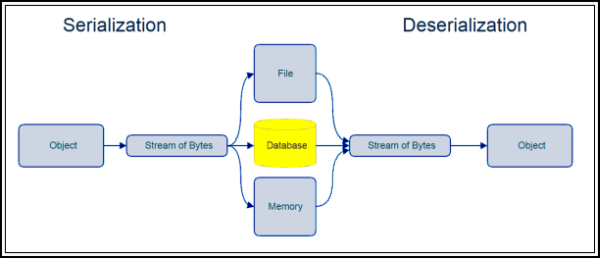
\includegraphics[width=\textwidth,height=\textheight,keepaspectratio]{figuras/data-serialization-deserialization.png}
  \caption{Processo de serialização e deserialização}
\end{figure}

Este processo, embora demande tempo, permitiu que aplicações fizessem o consumo de informações de forma distribuída, contribuindo com o aumento do volume de dados que circulam pela internet. Além disso, fez-se necessário a seleção adequada de formatos de serialização cuja estrutura não prejudique o desempenho de aplicações na busca por dados. \cite{SumarayMakki2012}

Segundo a Cisco Systems\footnote{
  Empresa de sistemas de rede.
}, no ano de 2015, houve um aumento de 21\% no volume de tráfego de dados registrados apenas por seus aparelhos. Sendo a categoria Web, Email e Data responsável por representar aproximadamente 7,558 petabytes de dados transmitidos por seus clientes durante um mês. \cite{Cisco2016}

Para suprir esta alta demanda, diversos formatos de serialização foram introduzidos para melhor atender os problemas de desempenho experienciados por serviços que disponibilizam dados serializados. Dentre eles, tempo de serialização e deserialização, tamanho de transferência, flexibilidade de uso, facilidade de leitura, automação, suporte para linguagem, entre outros. Contudo, cada formato possui seus prós e contras. \cite{Guller2016}

\begin{table}[ht!]
  \centering
  \resizebox{\columnwidth}{!}{
    \begin{tabular}{|c|c|c|c|c|}
      \hline
      Formato & Especificação & Codificação & Human-Readable & Esquema/IDL \\
      \hline
      XML & Padronizada & Textual & Sim & Sim \\
      JSON & Padronizada & Textual & Sim & Parcial \\
      YAML & Padronizada & Textual & Sim & Parcial \\
      Avro & Padronizada & Binário & Não & Sim \\
      Protocol Buffers & Padronizada & Binário & Parcial & Sim \\
      Thrift & Não Padronizada & Binário & Parcial & Sim \\
      \hline
    \end{tabular}
  }
  \caption{Comparação de formatos de serialização}
\end{table}

Para melhor entender o que define cada formato, será feito uma abordagem sobre as categorias de classificação usadas para estudar o comportamento dos formatos existentes hoje.

\subsection[Especificação]{Especificação}

Um formato pode ter sua especificação classificada como padronizada ou não padronizada. Uma especificação padronizada é regida por requisitos que auxiliam na reprodutibilidade do processo em outras linguagens para maximização da compatibilidade e minimização de erros. Ao contrário, dada uma linguagem de programação, não é garantido que sua implementação esteja seguindo os padrões e poderá ser considerado como não padronizada. \cite{McDermid1991}

\subsection[Codificação]{Codificação}

Codificação é o processo de sequenciamento de caracteres usado na redução da transmissão e armazenamento de dados. É possível classificar em dois tipos: textuais e binários. Formatos baseados em texto não são codificados para seu fácil acesso e podem ser lidos diretamente através de editores de texto. Já um formato binário faz o uso intensivo da codificação e decodificação para salvar espaço. \cite{Queiros2014}

\subsection[Human-Readable]{Human-Readable}

Ao representar estruturas de dados em formatos de serialização para que máquinas possam fazer a leitura, não é garantido, no entanto, que esta representação também seja legível por seres humanos.

Para que um formato seja human-readable, além de máquinas, pessoas devem conseguir ler e dizer o que está sendo representado mesmo fora de contexto. Para desenvolvedores, este detalhe é essencial no processo de debugging\footnote{
  Depuração é o processo de encontrar e reduzir defeitos num aplicativo de software ou mesmo em hardware.
}. Apesar do processo de serialização de dados não prever a ideia de escrita manual, se um formato é legível por pessoas então também é possível ser descrito por elas. Em geral, a maioria dos formatos baseados em texto são human-readable, enquanto os formatos binários não são. \cite{SumarayMakki2012}

Nota-se que a leitura de um formato é diferente de seu entendimento, uma vez que nem todos os formatos possuem maneiras de descrever seus metadados. Por exemplo, JSON é um formato baseado em texto e tem como objetivo a facilidade de uso e legibilidade por desenvolvedores. Contudo, nem sempre é possível identificar o que está sendo representado em suas estruturas. Através de extensões como JSON-LD e JSON Schema, é possível descrever meta informações para melhor entender o que está sendo representado sem perder a estrutura original do formato JSON.

\subsection[Esquema/IDL]{Esquema/IDL}

Com objetivo de entender o que está sendo representado, alguns formatos disponibilizam na sua especificação maneiras de descrever metadados. Esta categoria é importante principalmente para que máquinas consigam inferir quais estruturas estão sendo lidas e, assim, tomar decisões de forma autônoma.

Um formato descritivo normalmente disponibiliza estruturas como esquemas IDL\footnote{
  Linguagem de descrição utilizada para descrever a interface dos componentes de um software.
} para descrição da própria representação. À medida que estas descrições são incorporadas dentro da mesma representação, é possível classificar estes formatos como sendo auto-descritivos. \cite{Rentachintala2014}

